\chapter{Storage Devices and File Systems}\label{ch:b3:file-systems}

Memory forgets everything when the power goes; files must not. This chapter goes down to the devices that keep them, a disk whose head must travel and wait for the platter, a flash chip that cannot overwrite a page in place, and back up to the structures a file system builds on them: a \omterm{def:b3:file-systems:layout}{superblock}, bitmaps, inodes, blocks reached directly or through blocks of pointers, directories that are themselves files. A complete small file system, \code{minifs}, is written in C over an image file; then the machine is stopped in the middle of an update, at every possible moment, to see what a crash breaks and how a journal repairs it. Two last ideas make storage fast and safe at scale: writing everything as a log, and spreading data over several disks so that one can fail.

\begin{recall}
In the Year~2 volume a process reaches a file through a file descriptor, a small number the kernel gives it when it opens the file. The file itself is described by an inode, which holds its size, its owner, its permissions and where its data lie, but not its name: a name is an entry in a directory, a link to an inode, and an inode can have several. Earlier volumes described the hard disk and the SSD as the computer's lasting memory, and the exclusive or (XOR) of two bits as 1 when they differ.
\end{recall}

\section{Disks and flash}\label{sec:b3:file-systems:devices}

A hard disk stores bits as magnetised spots on spinning platters, read and written by a head at the end of an arm that moves across them.

\begin{omfigure}
\raisebox{-0.5\height}{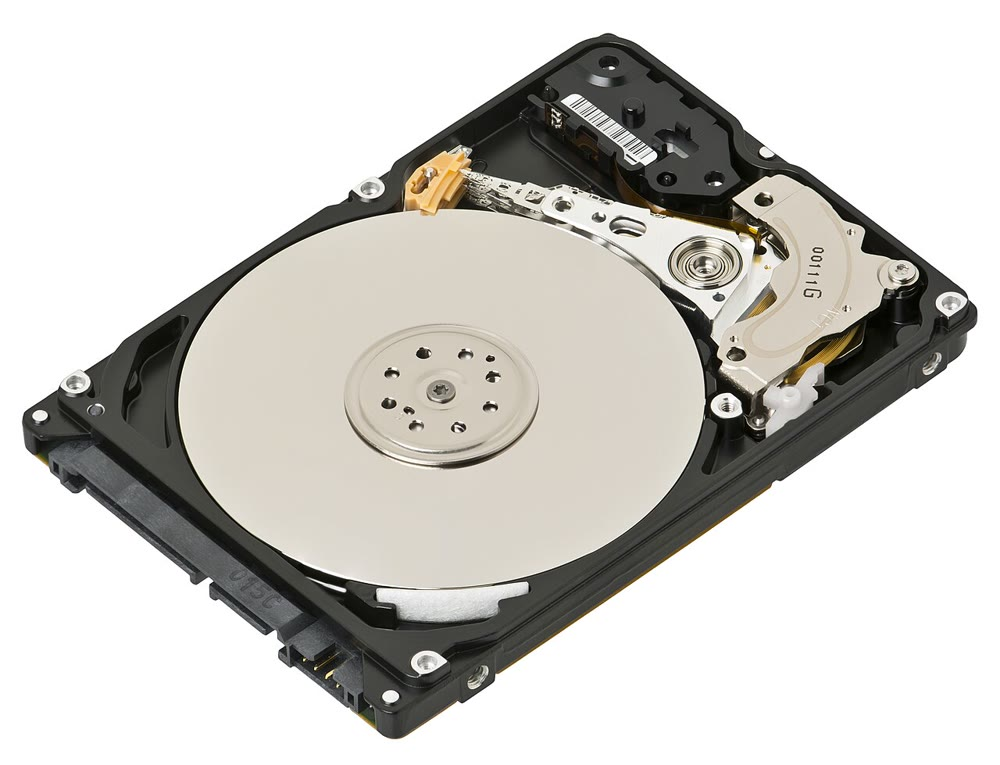
\includegraphics[width=0.44\linewidth]{images/book5/b3-12-hard-disk.jpg}}\hfill
\begin{tikzpicture}[font=\scriptsize, >=Stealth, baseline=(current bounding box.center)]
  \coordinate (c) at (0, 0);
  \fill[black!8] (0, 0) circle (2.1);
  \foreach \r in {0.7, 1.05, 1.4, 1.75} \draw[black!40] (0, 0) circle (\r);
  \fill[omThm!45] (0, 0) ++(20:1.4) arc (20:45:1.4) -- ++(45:0.35) arc (45:20:1.75) -- cycle;
  \fill[black!60] (0, 0) circle (0.25);
  \draw[very thick, black!70] (3.3, -1.6) -- (1.5, 0.75);
  \fill[omDef] (1.5, 0.75) circle (0.08);
  \fill[black!70] (3.3, -1.6) circle (0.12);
  \draw[->, omDef] (2.6, -0.9) arc (-60:-20:0.9);
  \node[align=left, anchor=west] at (2.2, 1.8) {sector: the smallest\\unit read or written};
  \draw[black!50] (2.2, 1.8) -- (1.2, 0.9);
  \node[anchor=north] at (0, -2.2) {track: one circle};
  \node[anchor=west] at (3.0, -0.9) {seek};
  \draw[->, black!60] (-1.9, 1.5) arc (140:100:1.6);
  \node[anchor=east] at (-1.9, 1.5) {rotation};
\end{tikzpicture}
\par\smallskip{\small Left: a 2.5-inch laptop hard disk, opened, with its platter and, at the right, the arm that carries the head. % ledger: b3:hd-photo
Right: the geometry. The arm moves the head to a track, a \emph{seek}; then the platter's rotation brings the wanted \omterm{def:b3:file-systems:disk}{sector} under it.}
\end{omfigure}

\begin{definition}[Disk block, sector, seek time, rotational latency]\label{def:b3:file-systems:disk}
A \emph{sector}\index{sector} is the smallest unit a disk reads or writes. A \emph{disk block}\index{disk block} is the unit a file system allocates and transfers, a fixed number of consecutive sectors. The \emph{seek time}\index{seek time} of an access is the time the arm takes to bring the head over the right track; the \emph{rotational latency}\index{rotational latency} is the time the platter then takes to bring the first sector under the head.
\end{definition}

The time of one access is the seek, plus the \omterm{def:b3:file-systems:disk}{rotational latency}, plus the transfer:
\[ T = t_{\text{seek}} + \frac{1}{2}\,\frac{60}{\mathit{rpm}} + \frac{\text{bytes}}{\text{transfer rate}}, \]
where on average the platter must turn half a revolution. For a hypothetical disk spinning at 7,200 revolutions per minute with an average seek of 9~ms, the \omterm{def:b3:file-systems:disk}{rotational latency} alone is 4.2~ms, and a read of 4~KiB at 150~MB/s takes 0.03~ms to transfer: almost all of the 13~ms goes to moving the mechanics, nothing to the data. A disk therefore reads large runs of consecutive blocks far faster than scattered ones, and the order in which it serves the requests waiting for it matters.

\begin{definition}[Disk scheduling, SCAN]\label{def:b3:file-systems:disk-scheduling}
\emph{Disk scheduling}\index{disk scheduling} chooses the order in which a disk serves the requests in its queue. \emph{Shortest \omterm{def:b3:file-systems:disk}{seek time} first} serves the request nearest to the head. The \emph{SCAN algorithm}\index{SCAN algorithm}, or elevator, moves the head in one direction to the last cylinder, serving every request on the way, then turns back and does the same in the other direction.
\end{definition}

\omcode{code/bachelor-3/12-file-systems/listings/disk_sched.py}{8}{41}{Three schedulers, and the distance the head travels. A cylinder is the set of tracks under the heads at one arm position.}\label{lst:b3:file-systems:sched}

\omoutput{code/bachelor-3/12-file-systems/outputs/disk_sched.txt}{Ten requests on a disk of 200 cylinders, the head at 100.}\label{out:b3:file-systems:sched}

Shortest \omterm{def:b3:file-systems:disk}{seek time} first travels least here, but it serves the requests near the head first, and a request far away can wait for ever while new ones keep arriving near the head; SCAN travels a little more and bounds every wait (exercise~\ref{exo:b3:file-systems:11}). A disk's own controller can reorder the requests it holds too, since it knows where the platter is.

Flash memory has no moving parts and no seek, but a constraint of its own. It is written by \emph{pages} of a few kilobytes, and a page can be written only once: to write it again, the whole \emph{\omterm{def:b3:file-systems:flash}{erase block}} that contains it, many pages, must first be erased.

\begin{definition}[Erase block, flash translation layer, wear levelling, write amplification]\label{def:b3:file-systems:flash}
An \emph{erase block}\index{erase block} is the smallest unit of flash that can be erased. The \emph{flash translation layer}\index{flash translation layer} (FTL) is the controller's software that maps the logical pages the computer writes to physical pages: an overwrite goes to a fresh page and the old copy becomes garbage, and \emph{cleaning} erases a block after copying out its pages still valid. \emph{Wear levelling}\index{wear levelling} spreads the erasures over all blocks, since each block survives a limited number of them. \emph{Write amplification}\index{write amplification} is the ratio of the pages written to the flash to the pages the computer asked to write.
\end{definition}

\omcode{code/bachelor-3/12-file-systems/listings/ftl.py}{8}{43}{An FTL over 64 \omterm{def:b3:file-systems:flash}{erase blocks} of 64 pages. It writes into one block at a time; when no erased block is left, it cleans the block with the fewest valid pages.}\label{lst:b3:file-systems:ftl}

\omoutput{code/bachelor-3/12-file-systems/outputs/ftl.txt}{\omterm{def:b3:file-systems:flash}{Write amplification} when a fraction $u$ of the flash holds data that the computer overwrites at random. The fraction of valid pages in the cleaned blocks predicts it exactly.}\label{out:b3:file-systems:ftl}

Cleaning a block whose fraction $v$ of pages is valid copies $vP$ pages to free $(1 - v)P$ for new data: each page the computer writes costs $1/(1 - v)$ pages of flash, which is the measured amplification to two decimals. Greedy cleaning chooses blocks emptier than the average, so the amplification stays far below $1/(1 - u)$; but it still grows without bound as the flash fills. In the model, two remedies lower $u$: keeping part of the flash hidden from the computer, and telling the drive which pages a deleted file no longer uses.

\begin{omfigure}
\begin{tikzpicture}
  \begin{axis}[omrecord, width=0.72\linewidth, height=5.2cm, xmin=0.48, xmax=0.92, ymin=0, ymax=10.5,
      xlabel={fraction $u$ of the flash in use}, ylabel={write amplification}, legend pos=north west,
      legend cell align=left]
    \addplot[omThm, thick, mark=*] table[x=u, y=wa] {code/bachelor-3/12-file-systems/figures/wa.dat};
    \addlegendentry{greedy cleaning, measured}
    \addplot[black!60, dashed, thick] table[x=u, y=average] {code/bachelor-3/12-file-systems/figures/wa.dat};
    \addlegendentry{cleaning a block of average use, $1/(1 - u)$}
  \end{axis}
\end{tikzpicture}
\par\smallskip{\small The cost of overwriting in place on flash, from \cref{out:b3:file-systems:ftl}. At 90~\% full, each page written costs 5.6 pages of flash.}
\end{omfigure}

\section{The layout of a file system}\label{sec:b3:file-systems:layout}

A file system turns a device, an array of blocks, into a tree of named files. Every Unix-like file system rests on the same few structures.

\begin{definition}[Superblock, block bitmap, inode table, direct and indirect blocks, directory entry]\label{def:b3:file-systems:layout}
The \emph{superblock}\index{superblock} describes the file system: its size and where its other structures lie. The \emph{block bitmap}\index{block bitmap} has one bit per block, set when the block is in use, and an inode bitmap does the same for inodes. The \emph{inode table}\index{inode table} holds the inodes, at fixed places, so that an inode number gives its position. An inode's \emph{direct blocks}\index{direct block} are the blocks whose numbers it holds itself; an \emph{indirect block}\index{indirect block} is a block that holds block numbers, reached from the inode. A \emph{directory entry}\index{directory entry} pairs a name with an inode number; a directory is a file whose data are its entries.
\end{definition}

\code{minifs} keeps 1,024 blocks of 1~KiB in an image file (\cref{lst:b3:file-systems:layout}): a \omterm{def:b3:file-systems:layout}{superblock}, the two bitmaps, eight blocks of inodes, a journal of 32 blocks for later, and the data. Its inode holds ten \omterm{def:b3:file-systems:layout}{direct block} numbers and one \omterm{def:b3:file-systems:layout}{indirect block} of 256 numbers.

\omcode{code/bachelor-3/12-file-systems/listings/minifs.h}{9}{22}{The layout, and an inode of 64 bytes.}\label{lst:b3:file-systems:layout}

\begin{omfigure}
\begin{tikzpicture}[font=\scriptsize, x=1mm, y=1mm]
  \foreach \a/\b/\l/\c in {0/12/{0}/black!25, 12/21/{1}/omDef!25, 21/30/{2}/omDef!25, 30/55/{3--10}/omThm!20,
                          55/85/{11--42}/omMeth!20, 85/140/{43--1023}/black!5} {
    \draw[fill=\c] (\a, 0) rectangle (\b, 8);
    \node at ({(\a + \b) / 2}, 4) {\l};
  }
  \node[below, align=center] at (6, 0) {super-\\block};
  \node[below, align=center] at (21, 0) {bitmaps};
  \node[below, align=center] at (42.5, 0) {inode table\\128 inodes};
  \node[below, align=center] at (70, 0) {journal\\(\cref{sec:b3:file-systems:crash})};
  \node[below, align=center] at (112.5, 0) {data blocks};
\end{tikzpicture}
\par\smallskip{\small The 1,024 blocks of a \code{minifs} image, by block number, from the first lines of \cref{out:b3:file-systems:demo} (not to scale). Block 1 is the inode bitmap, block 2 the \omterm{def:b3:file-systems:layout}{block bitmap}.}
\end{omfigure}

To find the $k$-th block of a file, \code{bmap} looks in the inode for $k < 10$, and otherwise in the \omterm{def:b3:file-systems:layout}{indirect block}; when asked to, it allocates the block, and the \omterm{def:b3:file-systems:layout}{indirect block} itself, on the way (\cref{lst:b3:file-systems:bmap}). Writing bytes is then a loop over blocks: find or allocate the block, read it if it is only partly overwritten, change it, write it; and at the end write the inode, with its new size and pointers (\cref{lst:b3:file-systems:write}).

\omcode{code/bachelor-3/12-file-systems/listings/minifs.c}{136}{156}{The file's $k$-th block. Allocating sets \code{*fresh}.}\label{lst:b3:file-systems:bmap}

\begin{omfigure}
\begin{tikzpicture}[font=\scriptsize, >=Stealth, x=10mm, y=5mm,
  s/.style={draw, minimum width=16mm, minimum height=5mm, inner sep=1pt},
  d/.style={draw, fill=black!6, minimum width=8mm, minimum height=5mm}]
  \node[font=\small] at (0, 1.4) {inode};
  \node[s, fill=omThm!12] at (0, 0.2) {type, size};
  \foreach \i/\l in {1/direct[0], 2/direct[1], 3/{\dots}, 4/direct[9], 5/indirect} \node[s, fill=omThm!12] (p\i) at (0, -\i + 0.2) {\l};
  \node[d] (b0) at (3, 1) {47};
  \node[d] (b1) at (3, -0.4) {48};
  \node[d] (b9) at (3, -2.4) {56};
  \draw[->] (p1.east) -- (b0.west);
  \draw[->] (p2.east) -- (b1.west);
  \draw[->] (p4.east) -- (b9.west);
  \node[draw, fill=omDef!12, minimum width=14mm, minimum height=18mm, align=center] (ind) at (3.2, -5.6) {256 block\\numbers};
  \draw[->] (p5.east) -- (ind.west);
  \node[d] (c0) at (6, -4.6) {58};
  \node[d] (c1) at (6, -5.8) {59};
  \node at (6, -6.8) {\dots};
  \draw[->] (ind.east) -- (c0.west);
  \draw[->] (ind.east) -- (c1.west);
  \node[anchor=west, align=left] at (6.6, -5.3) {file blocks 10 to 265:\\3 reads each, with the inode's};
  \node[anchor=west, align=left] at (3.6, -0.6) {file blocks 0 to 9:\\2 reads each};
\end{tikzpicture}
\par\smallskip{\small A \code{minifs} inode, with the block numbers of \code{big.dat} in \cref{out:b3:file-systems:demo}, whose \omterm{def:b3:file-systems:layout}{indirect block} is 57. Small files need only the inode; a larger file costs one more block, of pointers, and one more read for each of its blocks beyond the tenth. ext2's inode has 12 direct pointers and one single, one double and one triple indirect pointer, each level a tree one deeper. % ledger: b3:ext2-pointers
}
\end{omfigure}

\omcode{code/bachelor-3/12-file-systems/listings/minifs.c}{158}{186}{Writing bytes: the data blocks first, then the inode. \code{fs_write} wraps it in a transaction, which does nothing until the journal is on.}\label{lst:b3:file-systems:write}

A directory is a file of 32-byte entries, read and written by the same functions. Creating a file allocates an inode in the inode bitmap, writes the inode, and appends an entry to the directory (\cref{lst:b3:file-systems:create}).

\omcode{code/bachelor-3/12-file-systems/listings/minifs.c}{214}{228}{Creating a file: four block writes, in this order.}\label{lst:b3:file-systems:create}

\omcode{code/bachelor-3/12-file-systems/listings/fs_demo.c}{8}{35}{A file system in an image file: two files, a directory, a file in it, and a 12~KiB file.}\label{lst:b3:file-systems:demo}

\omoutput{code/bachelor-3/12-file-systems/outputs/fs_demo.txt}{The layout, a listing of each directory with inode numbers and blocks, and one file read back.}\label{out:b3:file-systems:demo}

Block 43, the first data block, is the root directory's; each file then takes the lowest free blocks. The 12~KiB file fills its ten \omterm{def:b3:file-systems:layout}{direct blocks}, and its last two blocks go behind the \omterm{def:b3:file-systems:layout}{indirect block}, 57.

\section{Crash consistency}\label{sec:b3:file-systems:crash}

Creating a file and writing 1,500 bytes into it makes nine block writes in \code{minifs}: the inode bitmap, the inode, the directory's data and the directory's inode, then for each of two data blocks the \omterm{def:b3:file-systems:layout}{block bitmap} and the block, and the file's inode. A disk writes one block at a time. If the power fails between two of those writes, the disk holds a state that no correct sequence of operations could have produced.

\begin{definition}[Crash consistency, journaling, idempotent replay]\label{def:b3:file-systems:consistency}
A file system has \emph{crash consistency}\index{crash consistency} when, whatever the moment the machine stops, the disk afterwards holds a consistent state: every block in use is marked in the bitmap and belongs to one file, every allocated inode is in a directory. \emph{Journaling}\index{journaling} achieves it by writing the blocks an operation will change first to a journal, then a commit record, and only then the blocks in place; after a crash, the committed operations are copied again from the journal. That \emph{replay} is \emph{idempotent}\index{idempotent replay}: replaying once or several times leaves the same state.
\end{definition}

A checker in the style of Unix's \code{fsck} finds the damage: it walks the directory tree from the root, marking every inode and block it reaches, and compares with the bitmaps (\cref{lst:b3:file-systems:check}). \Cref{lst:b3:file-systems:crash} stops the machine after each possible number of writes, reboots, and checks.

\omcode{code/bachelor-3/12-file-systems/listings/minifs.c}{346}{364}{The checker's verdict: the bitmaps against what the tree uses.}\label{lst:b3:file-systems:check}

\omcode{code/bachelor-3/12-file-systems/listings/crash.c}{31}{56}{A crash after each write in turn. \code{crash_at} makes every later write vanish.}\label{lst:b3:file-systems:crash}

\omoutput{code/bachelor-3/12-file-systems/outputs/crash.txt}{Without a journal: the blocks written, in order, then the state after each crash.}\label{out:b3:file-systems:crash}

The damage is only of one kind, an inode or a block marked in use that nothing uses: a leak, which a checker can repair by clearing the bit. That is because \code{minifs} writes in a careful order: the bitmap before the block it allocates, the block before the pointer to it, the inode before the \omterm{def:b3:file-systems:layout}{directory entry} that names it. The opposite order would leave a pointer to a block still free in the bitmap, which the next allocation would hand to another file: two files sharing a block, the worst damage of all. Careful ordering limits the damage; it does not prevent it, a checker must still read the whole disk after a crash, and a file of 0 bytes, created but never written, can survive a crash in the middle of an operation that should have written it whole.

A journal makes each operation all or nothing. \Cref{lst:b3:file-systems:commit} writes the operation's blocks to the journal, then a descriptor that lists where each belongs and carries the commit mark, in a single block write; then the blocks in place; then it clears the descriptor.

\omcode{code/bachelor-3/12-file-systems/listings/minifs.c}{51}{81}{Commit, and replay at mount: a journal block is copied home only if its descriptor carries the commit mark.}\label{lst:b3:file-systems:commit}

\begin{omfigure}
\begin{tikzpicture}[font=\scriptsize, x=15mm, y=6mm]
  \foreach \x/\l/\c in {0/{log 12}/omMeth!20, 1/{log 13}/omMeth!20, 2/{log 14}/omMeth!20, 3/{commit 11}/omThm!35,
                        4/{home 1}/black!8, 5/{home 3}/black!8, 6/{home 43}/black!8, 7/{clear 11}/omDef!20}
    \node[draw, fill=\c, minimum width=14.4mm, minimum height=6mm] at (\x, 0) {\l};
  \draw[omThm, very thick] (3.5, -0.9) -- (3.5, 0.9);
  \node[align=center, omThm] at (3.5, 1.6) {commit point};
  \node[align=center] at (1, -1.6) {crash here: the operation\\never happened};
  \node[align=center] at (5.5, -1.6) {crash here: replay\\completes it};
\end{tikzpicture}
\par\smallskip{\small The first transaction of \cref{out:b3:file-systems:journal}, creating \code{log.txt}: three blocks logged, the commit, three blocks written in place, the journal cleared. A crash before the commit loses the operation whole; after it, the replay at the next mount writes the three blocks again, whether or not they had already reached their place.}
\end{omfigure}

\omcode{code/bachelor-3/12-file-systems/listings/journal.c}{1}{4}{The same crashes, with the journal on.}\label{lst:b3:file-systems:journal}

\omoutput{code/bachelor-3/12-file-systems/outputs/journal.txt}{With a journal: twice as many writes, and a consistent disk after every crash. \code{log.txt} is absent, empty, or complete with its 1,500 bytes.}\label{out:b3:file-systems:journal}

Every block is written twice, which is the price. A file system can therefore journal only the metadata (bitmaps, inodes, directories) and write the data blocks in place; exercise~\ref{exo:b3:file-systems:12} shows why that order matters.

\section{Log-structured file systems}\label{sec:b3:file-systems:lfs}

\begin{definition}[Log-structured file system, segment cleaning]\label{def:b3:file-systems:lfs}
A \emph{log-structured file system}\index{log-structured file system} writes every change, data and metadata alike, at the end of a log, in large sequential segments, never in place; an inode map records where the latest copy of each inode is. \emph{Segment cleaning}\index{segment cleaning} reclaims space: it reads a segment, writes its blocks that are still live at the end of the log, and frees the segment.
\end{definition}

On a disk, writing whole segments turns every write into a sequential one, the fastest kind; and a crash can only cut the end of the log. The cost is cleaning, the same mechanism as an FTL's, with the same algebra: cleaning segments that are a fraction $u$ live costs, per block of new data, the reading of the segment, the writing of its live blocks and the writing of the new block, $2/(1 - u)$ blocks of disk traffic (exercise~\ref{exo:b3:file-systems:10}). Mendel Rosenblum and John Ousterhout published the design of such a file system in 1992. % ledger: b3:rosenblum-ousterhout-1992
An FTL like \cref{lst:b3:file-systems:ftl}'s is itself log-structured, whatever file system runs above it.

\section{Redundancy across disks}\label{sec:b3:file-systems:raid}

\begin{definition}[RAID, striping, mirroring, parity block]\label{def:b3:file-systems:raid}
\emph{RAID}\index{RAID} (redundant array of independent disks) presents several disks as one. \emph{Striping}\index{striping} spreads consecutive blocks over the disks, so that a large transfer uses all of them at once (RAID 0, no redundancy). \emph{Mirroring}\index{mirroring} keeps a copy of every block on two disks (RAID 1). A \emph{parity block}\index{parity block} holds the XOR of the blocks of one stripe on the other disks, so that any one of them can be rebuilt as the XOR of the others (RAID 5, with the parity moving from disk to disk).
\end{definition}

If $p = d_0 \oplus d_1 \oplus d_2 \oplus d_3$, then $d_1 = d_0 \oplus d_2 \oplus d_3 \oplus p$, since $x \oplus x = 0$: the lost block is the XOR of the survivors.

\omcode{code/bachelor-3/12-file-systems/listings/raid5.py}{9}{35}{Parity, \omterm{def:b3:file-systems:raid}{striping} with rotating parity, and reading back.}\label{lst:b3:file-systems:raid}

\omoutput{code/bachelor-3/12-file-systems/outputs/raid5.txt}{The first five stripes, the data's digest, and the digest after disk 2 is lost and rebuilt.}\label{out:b3:file-systems:raid}

The parity moves so that no disk becomes the bottleneck: every small write must also update its stripe's parity. \omterm{def:b3:file-systems:raid}{RAID} 6 adds a second, independent redundancy block per stripe, to survive two failures. How safe is \omterm{def:b3:file-systems:raid}{RAID} 5? Suppose each of $N$ disks fails at random, with a mean time to failure $M$, and that a failed disk is replaced and rebuilt in a time $R$ much shorter than $M$. A first failure comes after $M/N$ on average; data are lost only if one of the $N - 1$ others fails during the $R$ hours of rebuilding, which happens with probability about $(N - 1)R/M$. The mean time to data loss is about
\[ \frac{M/N}{(N - 1)R/M} = \frac{M^2}{N(N - 1)R}, \]
the square of the disks' lifetime: that is the gain of a single \omterm{def:b3:file-systems:raid}{parity block}. The model assumes independent failures; disks bought together, in the same box, fail together more often than it says. David Patterson, Garth Gibson and Randy Katz made the case for arrays of inexpensive disks in 1988. % ledger: b3:patterson-gibson-katz-1988

\begin{history}[Storage]
Patterson, Gibson and Katz's \emph{A case for redundant arrays of inexpensive disks} appeared at SIGMOD in 1988, % ledger: b3:patterson-gibson-katz-1988
and Rosenblum and Ousterhout's \omterm{def:b3:file-systems:lfs}{log-structured file system} in the ACM Transactions on Computer Systems in February 1992. % ledger: b3:rosenblum-ousterhout-1992
\end{history}

\section{Exercises}\label{sec:b3:file-systems:exercises}

\begin{exercise}[$\star$]\label{exo:b3:file-systems:1}
A hypothetical disk turns at 7,200 rpm, seeks in 9~ms on average and transfers 150~MB/s. How long does reading 4~KiB at a random place take? And 4~MiB?
\end{exercise}

\begin{exercise}[$\star$]\label{exo:b3:file-systems:2}
The head is at cylinder 50, moving up, on a disk of 200 cylinders; the queue holds 82, 17, 43, 140, 24, 16 and 190. Give SCAN's order and the distance the head travels.
\end{exercise}

\begin{exercise}[$\star$]\label{exo:b3:file-systems:3}
How many blocks, and of which kinds, does a file of 50~KiB use in \code{minifs}?
\end{exercise}

\begin{exercise}[$\star$]\label{exo:b3:file-systems:4}
After \cref{lst:b3:file-systems:demo}, the program unlinks \code{notes.txt}, then creates \code{todo.txt} and writes 3 bytes in it. Which inode and which block does \code{todo.txt} get, and where does it appear in the root's listing?
\end{exercise}

\begin{exercise}[$\star\star$]\label{exo:b3:file-systems:5}
A first version of \code{fs_unlink} is below. After it removes a file of 3,000 bytes, the checker reports three problems. Which ones, and what is missing?

\omcode{code/bachelor-3/12-file-systems/exercises/ex5_unlink_bug.c}{2}{19}{\code{unlink}, as first written.}\label{lst:b3:file-systems:unlinkbug}
\end{exercise}

\begin{exercise}[$\star\star$]\label{exo:b3:file-systems:6}
Give \code{minifs} a double-indirect pointer, the field \code{dindirect}: write \code{bmap_double(in, k, fresh)}, which \code{bmap} calls for the blocks beyond the \omterm{def:b3:file-systems:layout}{indirect block}'s when \code{DOUBLE_INDIRECT} is defined. How many reads does a byte at 290~KiB then cost?
\end{exercise}

\begin{exercise}[$\star\star$]\label{exo:b3:file-systems:7}
Prove that the replay of \cref{lst:b3:file-systems:commit} is \omterm{def:b3:file-systems:consistency}{idempotent}, and that after a crash at any moment, followed by a replay (itself possibly interrupted by crashes), the disk holds either the state before the operation or the state after it.
\end{exercise}

\begin{exercise}[$\star\star$]\label{exo:b3:file-systems:8}
How many block reads does \code{fs_read} make to read one byte at offset $k$ of a \code{minifs} file, given its inode number? Check against \cref{out:b3:file-systems:reads}.
\end{exercise}

\begin{exercise}[$\star\star$]\label{exo:b3:file-systems:9}
One stripe of a \omterm{def:b3:file-systems:raid}{RAID} 5 holds the data bytes \code{0x3C}, \code{0xA5}, \code{0x0F} and \code{0x81}. Compute the parity byte, then rebuild \code{0xA5} after its disk is lost.
\end{exercise}

\begin{exercise}[$\star\star\star$]\label{exo:b3:file-systems:10}
A \omterm{def:b3:file-systems:lfs}{log-structured file system} cleans segments whose fraction $u$ of blocks is live, reading each segment whole. Show that writing new data costs $2/(1 - u)$ blocks of disk traffic per block of new data, and $1$ when $u = 0$. Why can it be worth cleaning segments that are not the emptiest?
\end{exercise}

\begin{exercise}[$\star\star\star$]\label{exo:b3:file-systems:11}
Show that shortest \omterm{def:b3:file-systems:disk}{seek time} first can make a request wait for ever, while SCAN serves every request within two sweeps of the disk; bound the head's travel before a request on a disk of $C$ cylinders is served.
\end{exercise}

\begin{exercise}[$\star\star\star$]\label{exo:b3:file-systems:12}
Metadata \omterm{def:b3:file-systems:consistency}{journaling} logs only bitmaps, inodes and directories; the data blocks are written in place, outside the journal. Show the crash that metadata \omterm{def:b3:file-systems:consistency}{journaling} allows if a new data block is written after the commit, and explain why writing data blocks in place before the commit, the \emph{ordered} mode, prevents it.
\end{exercise}

\section{Weekend problem}\label{sec:b3:file-systems:problem}

\begin{problem}[{Weekend problem --- How big can a file be?}]\label{pb:b3:file-systems:1}
The size of an inode's pointers decides how large a file can grow and how many reads it costs to reach its last byte. This problem computes both for a classic inode, measures them on \code{minifs}, and compares with extents.

\omcode{code/bachelor-3/12-file-systems/listings/max_file.py}{1}{28}{The largest file, region by region, for 12 direct pointers and one single, one double and one triple indirect pointer.}\label{lst:b3:file-systems:max}

\omoutput{code/bachelor-3/12-file-systems/outputs/max_file.txt}{The regions of the file for three block sizes.}\label{out:b3:file-systems:max}

\omcode{code/bachelor-3/12-file-systems/listings/file_reads.c}{7}{29}{\code{minifs} measured: fill a file until the pointers run out, then count the reads of one byte.}\label{lst:b3:file-systems:reads}

\omoutput{code/bachelor-3/12-file-systems/outputs/file_reads.txt}{The largest \code{minifs} file, and the reads per byte.}\label{out:b3:file-systems:reads}

\needspace{4\baselineskip}\medskip\noindent\textbf{Part I --- The classic inode.}
\begin{enumerate}
\item With blocks of 4~KiB and block numbers of 4 bytes, how many block numbers does a pointer block hold?
\item How many bytes are reached through the 12 direct pointers, and through the single, double and triple indirect pointers?
\item Give the largest file exactly, in bytes, and check it against \cref{out:b3:file-systems:max}.
\item Which part of the file dominates, and why does that make the direct pointers almost irrelevant to the maximum?
\item ext2 uses blocks of 1, 2 or 4~KiB, % ledger: b3:ext2-blocksize
and its documentation gives file size limits of 16~GB, 256~GB and 2,048~GB for them. % ledger: b3:ext2-file-limit
Which of these limits does the pointer tree explain?
\item Suppose the inode also counts the file's size in units of 512 bytes, in a 32-bit field. What limit results, and which block size does it constrain?
\end{enumerate}

\needspace{4\baselineskip}\medskip\noindent\textbf{Part II --- Reads per access.}
\begin{enumerate}[resume]
\item Without caching, how many block reads reach a byte in each region, and what is read each time?
\item In which region is the byte at offset 1~GiB, and what does reading it cost?
\item And the byte at offset 10~GiB?
\item Reading a 4~GiB file from start to end, how many pointer blocks are read, and what fraction of all the reads is that?
\item With every pointer block kept in memory, what does a read at a random offset cost?
\item Why must the inode be read too, and where is it found from its number?
\end{enumerate}

\needspace{4\baselineskip}\medskip\noindent\textbf{Part III --- \code{minifs} measured.}
\begin{enumerate}[resume]
\item Predict \code{minifs}'s largest file from its inode, and compare with \cref{out:b3:file-systems:reads}.
\item Explain the 2 and 3 block reads.
\item How many blocks of the disk does the largest file use, pointer block included?
\item What does the \code{fs_write} that finally returns 0 do, and why does it leave the disk consistent?
\item With exercise~\ref{exo:b3:file-systems:6}, how large could a file be, and what limits it first on this image?
\end{enumerate}

\needspace{4\baselineskip}\medskip\noindent\textbf{Part IV --- Extents.}
\begin{enumerate}[resume]
\item An \emph{extent} describes a run of consecutive blocks by its first block and its length. How many extents describe a 4~GiB file written in one run on an empty disk, and how many pointer bytes did the classic inode need for it?
\item What is the worst case for extents, and how does it compare with pointers?
\item With the extents sorted by file offset in the inode, how many reads reach any byte, and how is the extent found?
\item Why do extents also help the disk, beyond saving space?
\item For a file of 3~KiB, which representation is better, and does it matter?
\item Sum up: how big can a file be with the classic inode and 4~KiB blocks, what does its last block cost to reach, and what do extents change?
\end{enumerate}
\end{problem}
